\section{Exploration of Energy Storage Sizing} \label{sec:c3_exploration}

% The sizing method finds the suitable energy harvester size that achieves a target forward progress and explores the energy storage sizing effect (\sref{subsec:harvstor}), with a trade-off in forward progress, capacitor volume, and interruption periods (\sref{subsec:tradeoff}).

In this section, we present an exploration of the relationship between \nm{\alpha}{exe} and $C$ with respect to supply current \nm{I}{harv} and volatile state size.

\subsection{Impact of Supply Current} \label{subsec:sizees}

\begin{figure}
    \centering
    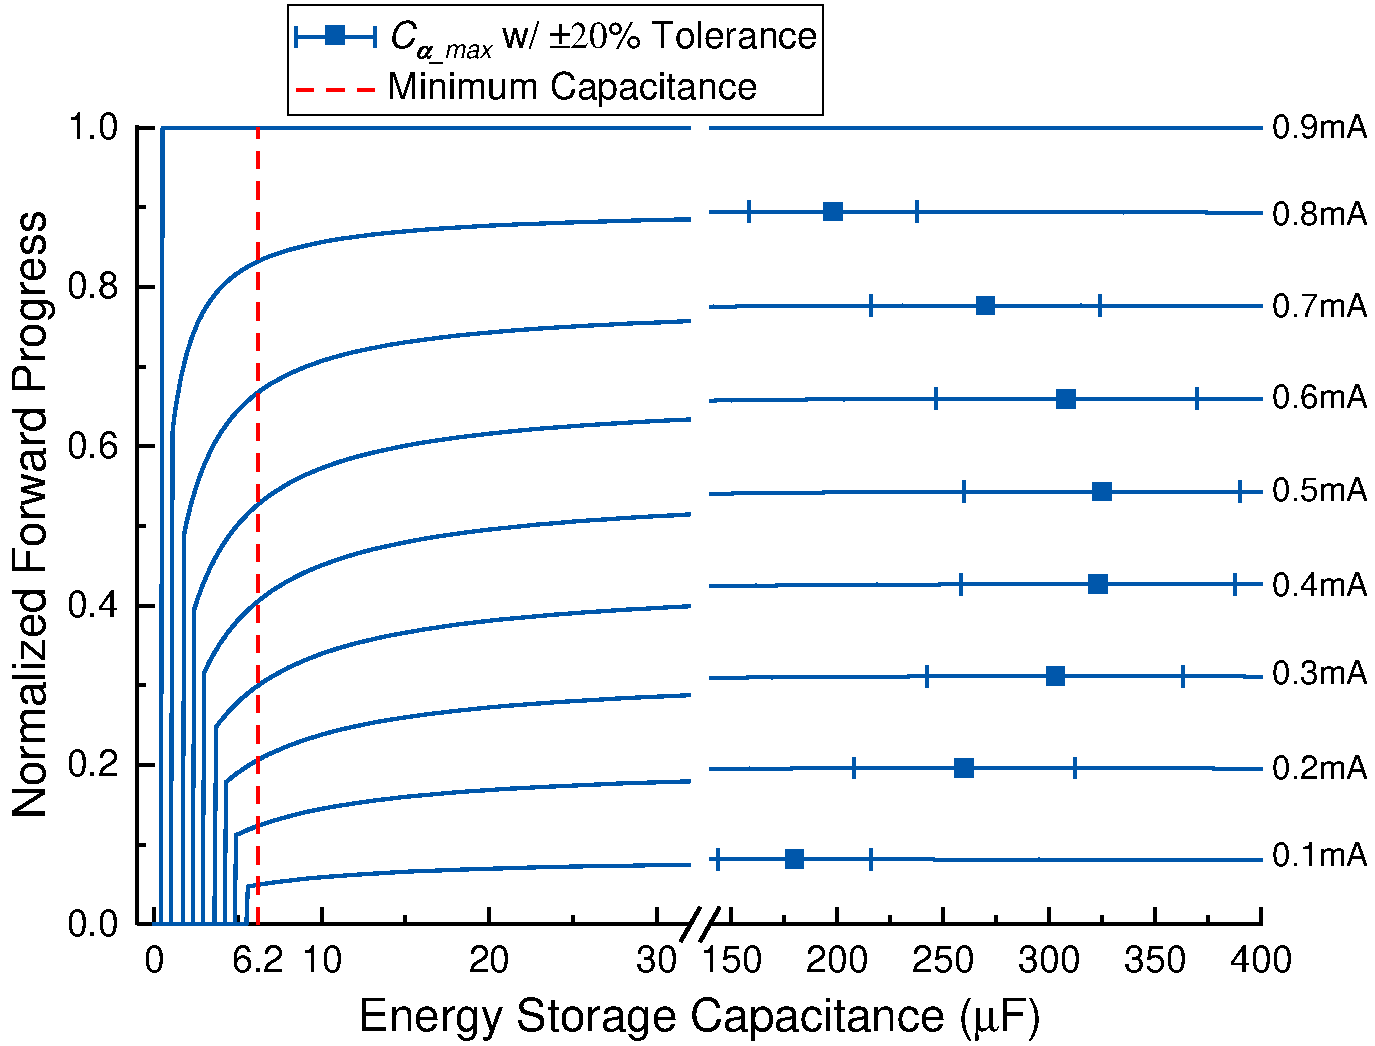
\includegraphics[width=\columnwidth]{ch3_sizingeffect/figures/StorCCur6Fig} 
    \caption{Forward progress against energy storage capacitance at different levels of constant supply current. Error bars around \nm{C}{$\alpha$\_max} denote the impact of typical $\pm$20\% capacitance tolerance. The \SIrange{30}{150}{\micro\farad} range is omitted as forward progress in that range increases monotonically. }
    \label{fig:fpwconstcurr}
\end{figure}

Increasing energy storage capacitance beyond the minimum one can improve forward progress by reducing the frequency of power interruptions, but this improvement may be offset by increased leakage. 
\fref{fig:fpwconstcurr} shows the relationship between forward progress and energy storage capacitance for a range of constant supply currents. 
In this section, we denote the capacitance that leads to the maximum forward progress \nm{\alpha}{exe} as \nm{C}{$\alpha$\_max}. 
\nm{C}{$\alpha$\_max} for each current value is also shown in \fref{fig:fpwconstcurr}.

% some more explanation about details in this graph
The minimum capacitance (dashed line in \fref{fig:fpwconstcurr}) is calculated to deliver correct operation even if the supply current instantaneously drops to zero. 
If it does not drop to zero, this means that correct operation could have continued even with a smaller capacitance given that the current supply keeps providing energy during execution, though designing a system in this way would be inadvisable owing to unpredictability of the supply. 
This property is illustrated in \fref{fig:fpwconstcurr}, in the area on the left of the dashed line. 
It may be observed that, for each of the current values, there is a sudden drop-off towards zero forward progress. 
This illustrates the hazard of setting the capacitance too small: the stored energy is too low to allow a restore and save to be undertaken.
The reason for this step change rather than a continuous change is that the implemented IPS only performs one restore operation in the first execution cycle after a reboot and enters a low-power mode with volatile state retained after a save operation. 
Hence the energy used for restoring state is then used for effective execution in the following operating cycles as long as the supply voltage recovers to the restore threshold without a power interruption.
% If the volatile state is not retained in low-power mode (i.e. necessary to restore every operating cycle) or the supply only lasts for a limited period, 
 
Typically, commercially-available capacitors have a $\pm$20\% tolerance. 
The effect of this variation on maximum forward progress is shown to be negligible ($<$ 0.23\%) in \fref{fig:fpwconstcurr}. 
However, it must be pointed out that the effect would be much more pronounced if operating at the minimum capacitance as the variation of forward progress is larger with smaller capacitance values. 
Thus, it is recommended that a tolerance is considered when designing IPSs with minimum capacitance.

\begin{figure}
    \centering
    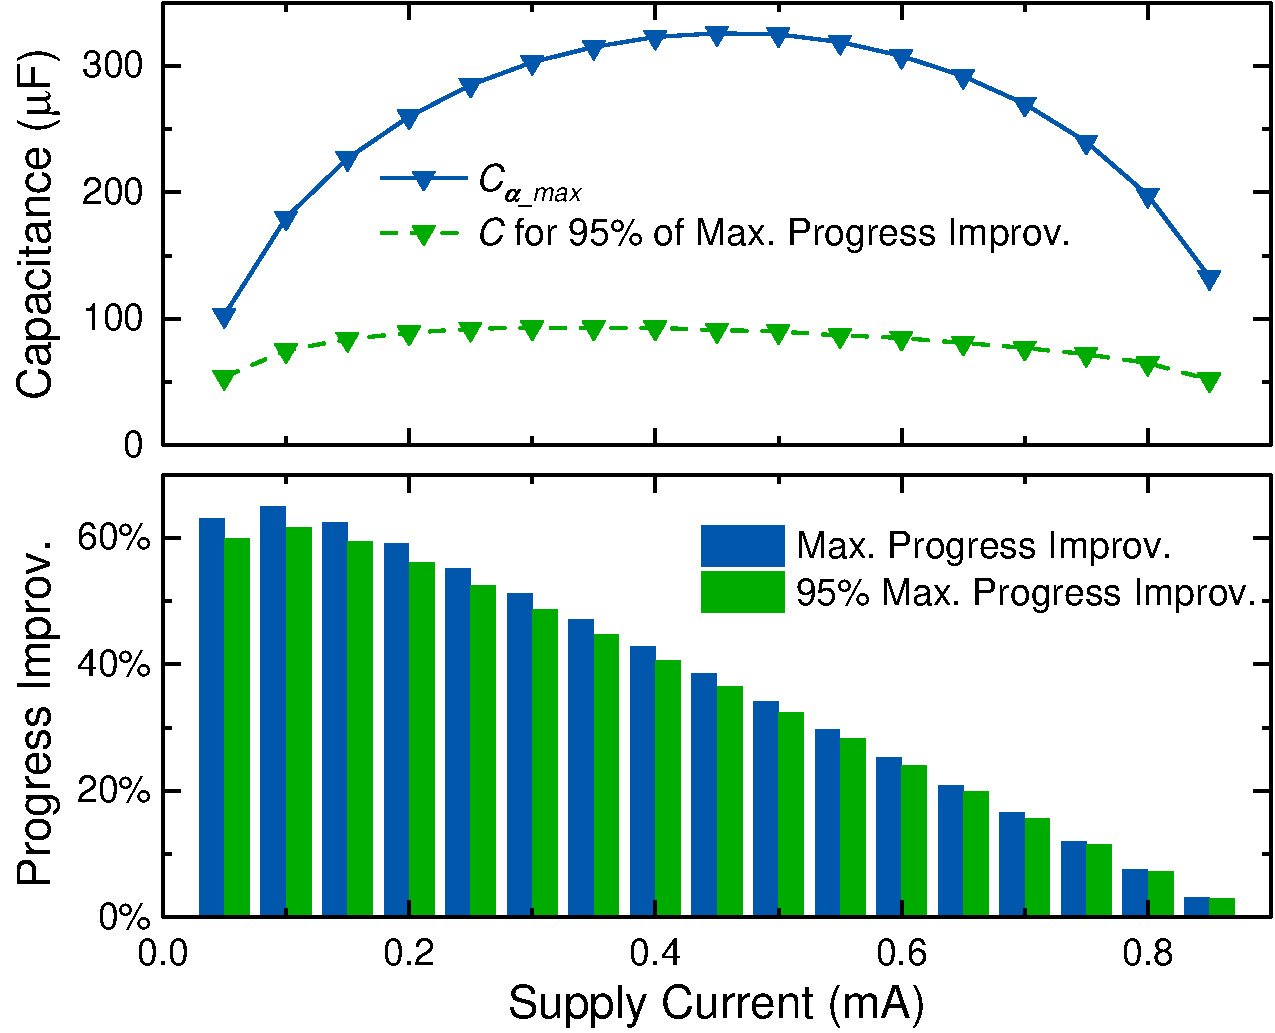
\includegraphics[width=\columnwidth]{ch3_sizingeffect/figures/StorCCurMax4Fig}
    \caption{Maximum forward progress improvement by sizing energy storage given a spectrum of supply current (normalised by the minimum capacitance case), with the corresponding capacitance for maximum and sub-maximum (95\% of maximum) forward progress improvement. }
    \label{fig:maxfwp}
\end{figure}

\fref{fig:maxfwp} shows that an improvement in forward progress of up to 65\%  can be achieved when using \nm{C}{$\alpha$\_max} instead of the minimum. 
However, it may not be desirable to set the capacitance solely for maximising forward progress, because there are often trade-offs with other factors including increased interruption periods and dimensions (later explored in \sref{subsec:tradeoff}).
In real-world energy source conditions, the supply current varies across this spectrum, and hence leads to an overall progress improvement based on its supply distribution. 
This improvement exists only when the device operates in the \textit{Intermittent} mode, since the device keeps either inactive in the \textit{Off} mode or active in the \textit{On} mode without the need for restoring and saving state. 
Correspondingly, \nm{C}{$\alpha$\_max} is also plotted against supply current. 
% This optimal capacity exists because of the side effect of capacitor leakage; without capacitor leakage effect, the forward progress would keep approaching the ideal case (as explained in \sref{subsec:formulation}). 
While a large improvement can be delivered with \nm{C}{$\alpha$\_max}, as shown in \fref{fig:maxfwp}, 95\% of this gain can still be obtained with significantly smaller capacitances (mean 31\% of \nm{C}{$\alpha$\_max}).
For example, reducing from \SI{325}{\micro\farad} to \SI{90}{\micro\farad} gives 95\% of the maximum improvement with a \SI{0.5}{\milli\ampere} supply. 

\subsection{Impact of Volatile State Size}

The size of volatile state differs across applications with different amounts of RAM usage, and hence incurs varying time and energy overheads for restore and save operations. 
We measured time overheads of restore and save operations in the minimum case (64B register data and a 160B stack) and the maximum case (64B register data and a full 2048B RAM) respectively as shown in \tref{tab:ramscale}. 
As these time overheads are expected to be linear to the state size~\cite{sliper2019efficient}, the model can be tuned for various volatile state sizes by linearly scaling the profiled values. 

\begin{table}
    \renewcommand{\arraystretch}{1.2}
    \centering
    \begin{tabular}{|c|cc|}
        \hline
        \textbf{State Size} & \multirow{2}{*}{\textbf{Restore Time}} & \multirow{2}{*}{\textbf{Save Time}}\\
        \textbf{(Registers + SRAM)} & & \\
        \hline
        64B + 160B (lower bound) & \SI{232}{\micro\second} & \SI{208}{\micro\second}\\
        % 64B registers + 160B stack
        64B + 2048B (upper bound) & \SI{2.298}{\milli\second} & \SI{2.274}{\milli\second} \\
        % 64B registers + 2048B RAM
        \hline
    \end{tabular}
    \caption{Linear scaling range of volatile state size and restore/save time overheads.}
    \label{tab:ramscale}
\end{table}

An example of this is plotted in \fref{fig:ram}. 
The forward progress improvement by sizing energy storage increases with the volatile state size, and \nm{C}{$\alpha$\_max} grows accordingly. 
The improvement becomes insignificant when the volatile state size is small because the restore and save overheads are already negligible. 
For example, when the workload uses the least volatile state (the leftmost point), the maximum progress improvement is only 3.6\% although the restore and save overheads are reduced by 93\%. 
% This indicates the more efficiently IPSs save/restore, the more useless this work is :p 

\begin{figure}
    \centering
    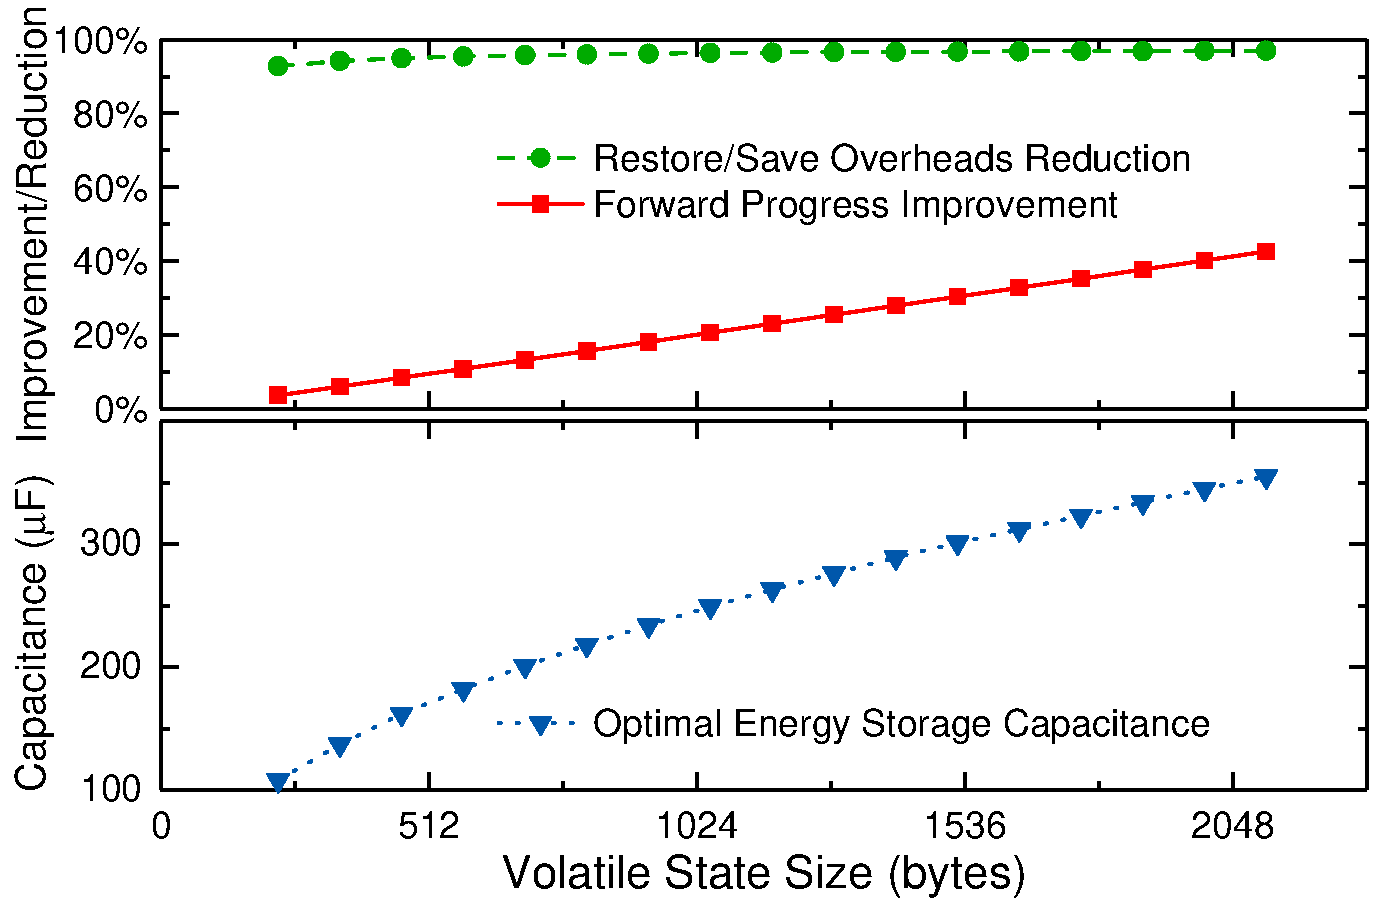
\includegraphics[width=\columnwidth]{ch3_sizingeffect/figures/RSTORAM3Fig}
    \caption{Impact of RAM usage (linear to restore/save overheads) on sizing energy storage with \SI{0.4}{\milli\ampere} current supply. Improvement and reduction are normalised by the minimum capacitance case. }
    \label{fig:ram}
\end{figure}

Where the size of the volatile state may vary at run time, a different capacitor size within the range \SIrange{108}{355}{\micro\farad} may have been recommended (\fref{fig:ram}). 
However, as can be seen from \fref{fig:fpwconstcurr}, there is a minimal difference in forward progress across this range. 
In the worst case, a 2.7\% reduction results from setting \nm{C}{$\alpha$\_max} for the minimum state size, while running with the largest state size.
